\documentclass[12pt,oneside,slovak,a4paper]{article}

\usepackage[slovak]{babel}
\usepackage[utf8]{inputenc}
\usepackage{amsmath}
\usepackage{amsfonts}
\usepackage{amssymb}
\usepackage{graphicx}
\usepackage{cite}
\usepackage[IL2]{fontenc} % lepšia sadzba písmena Ľ než v T1
\usepackage{pdfpages}
\usepackage{url} % príkaz \url na formátovanie URL
\usepackage[hidelinks]{hyperref} % odkazy v texte budú aktívne (pri niektorých triedach dokumentov spôsobuje posun textu)
\usepackage[left=2cm,right=2cm,top=2cm,bottom=2cm]{geometry}
\usepackage{float}
\usepackage[normalem]{ulem}
\useunder{\uline}{\ul}{}
\usepackage{titling}
\usepackage{xcolor}
\usepackage{lipsum}
\usepackage{setspace}
\usepackage{blindtext}
\usepackage{caption}
\usepackage{tabularx}
\usepackage[numbers]{natbib}




% riadkovanie 1.5
\begin{document}
\linespread{1.5}\selectfont

\begin{titlepage}
	\centering
    {\Large Slovenská technická univerzita v Bratislave\par}
    {\Large Fakulta informatiky a informačných technológií\par}
	\vspace{7cm}
	{\huge\bfseries Spoľahlivý systém ukladania osobných dát v domácnosti\par}
	\vspace{0.5cm}
    {\Large \textsc{Projektovanie aplikácií počítačov}\par}
    \vspace{1cm}
	{\Large\itshape Marek Čederle\par}
    {\small\texttt{xcederlem@stuba.sk}\par}
	\vfill

	{\large \today\par}
\end{titlepage}


% ----------------- Obsah -----------------
\tableofcontents
\vspace*{\fill}
\newpage

% ----------------- Kapitoly -----------------

% vsetky zdroje z literatura.bib aby sa zobrazili bez citovania
\nocite{*}

\section{Úvod}
V dobe, kedy digitálne údaje sú veľmi dôležité nielen pre firmy, ale aj pre jednotlivcov, je nevyhnutné mať spoľahlivé riešenie na ukladanie a zálohovanie údajov. Tento projekt sa zameriava na implementáciu spoľahlivého systému ukladania a zálohovania údajov, ktorý môže bežná osoba prevádzkovať v pohodlí svojho domova. Pôjde o vytvorenie systému NAS\footnote{Network Attached Storage} využívajúcej bežne dostupné počítačové komponenty a sieťovú infraštruktúru. Projekt sa venuje aj výberu vhodného softvéru, ktorý efektívne využije možnosti systému NAS. Okrem toho sa zaoberá umiestnením NAS v domácom prostredí, aby bolo zabezpečené pohodlné používanie bez zbytočného rušenia. Dôležitou súčasťou projektu je aj porovnanie nákladov medzi domácou a komerčnou alternatívou.

\section{Hardvér}
Z dôvodu aby sme čo najviac ušetrili peniaze a pomohli planéte pomocou toho že sa budeme riadiť podľa hesla ``Reduce, Reuse, Recycle'' sme sa rozhodli že použijeme starý počítač s relatívne novými komponentami, ktorý máme doma. Tento počítač bude slúžiť ako základ pre náš NAS systém na ktorom môžeme stavať ďalej alebo ho prípadne vylepšiť.

\subsection{PC Skriňa}


\begin{figure}[H]
	\centering
	\captionsetup{justification=centering,margin=2cm}
	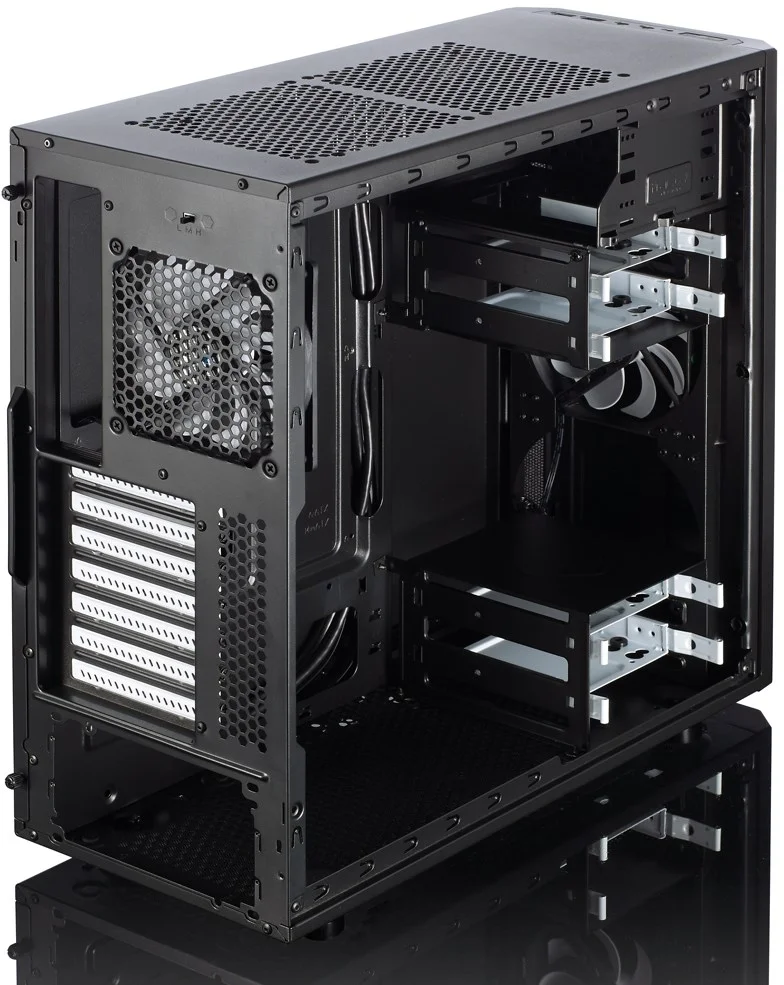
\includegraphics[scale=0.4]{./images/case.png}
	\centering
	\caption{Fractal Design CORE 2500 \\ Zdroj: https://www.alza.sk/fractal-design-core-2500-d2169926.htm}
\end{figure}

\begin{table}[h]
\centering
\begin{tabular}{|l|l|}
\hline
\textbf{Parameter} & \textbf{Value} \\ \hline
Veľkosť & Midi Tower \\ \hline
Farba & Čierna \\ \hline
Formát základnej dosky & ATX, mATX (Micro ATX), mITX (Mini ITX) \\ \hline
Počet interných 3,5" slotov & 4× \\ \hline
Počet interných 2,5" slotov & 1× \\ \hline
Max. výška chladiča procesora & 162 mm \\ \hline
Max. dĺžka grafickej karty & 380 mm \\ \hline
Ďalšie vybavenie & Prachové filtre \\ \hline
Externá 5,25" pozícia & 2× \\ \hline
Umiestnenie predného panelu & Zhora \\ \hline
Konektory predného panelu & USB 3.2 Gen 1, Slúchadlá, Mikrofón \\ \hline
Bočnica & Nepriehľadná \\ \hline
Materiál bočnice & Oceľová \\ \hline
Regulácia ventilátorov & Áno \\ \hline
Zdroj & Bez zdroja \\ \hline
Podporovaný formát zdroja & ATX \\ \hline
Veľkosť predného ventilátora & 1x120mm, 2x140mm \\ \hline
Veľkosť zadného ventilátora & 1x120mm \\ \hline
Veľkosť horného ventilátora & 1x120mm, 1x140mm \\ \hline
Počet pozícií pre ventilátory & 7× \\ \hline
Počet osadených ventilátorov & 2x120mm \\ \hline
Podporovaná veľkosť radiátora zhora & 120mm, 240mm \\ \hline
Podporovaná veľkosť radiátora spredu & 120mm, 140mm, 240mm, 280mm \\ \hline
Farba podsvietenia & Bez podsvietenia \\ \hline
Materiál skrine & Oceľ \\ \hline
Šírka & 195 mm (19,5 cm) \\ \hline
Výška & 431 mm (43,1 cm) \\ \hline
Hĺbka & 450 mm (45 cm) \\ \hline
Hmotnosť & 5,7 kg \\ \hline
\end{tabular}
\caption{PC Skriňa - Fractal Design CORE 2500}
\end{table}

\subsection{Základná doska}

\subsection{Procesor}

\subsection{Pamäť}

\subsection{Disky}
\subsubsection{Bootovací Disk}

\subsubsection{Úložné disky}


\subsection{Zdroj}

\subsection{Sieťová karta}

\subsection{Záložný zdroj v podobe UPS}

\section{Softér}

\subsection{RAID}

\subsection{Operačný systém}
TrueNAS or open media vault
Setupnut SMB na sieti na pristup

\section{Umiestnenie v domácnosti}
V naš

\begin{spacing}{1.0}
Legenda:
\begin{itemize}
	\item Zelenou farbou je označený router.
	\item Červenou farbou je označený sýstém NAS.
	\item Modrou farbou sú označené sieťové káble ktoré vedú ku zariadeniam cez rohovú lištu.
	\item Oranžovou farbou je označený domáci počítač.
\end{itemize}
\end{spacing}

\begin{figure}[H]
	\centering
	\captionsetup{justification=centering,margin=2cm}
	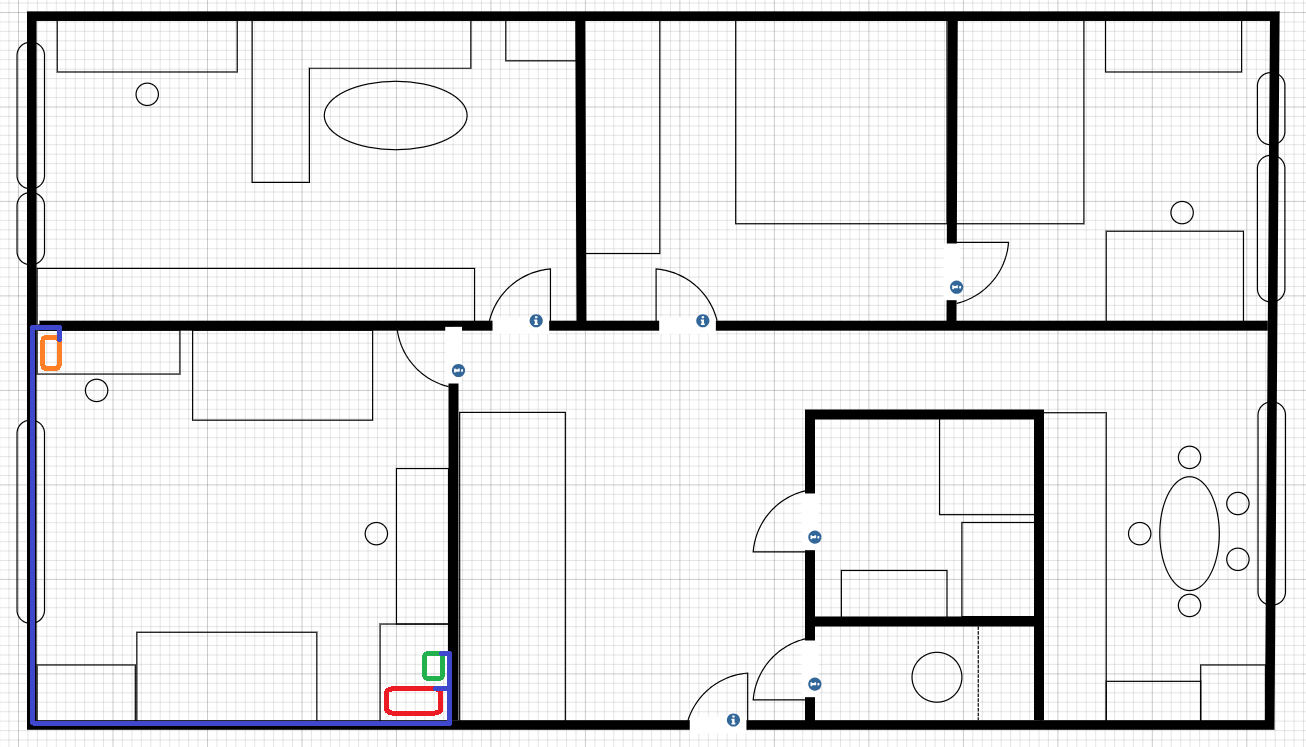
\includegraphics[width=\linewidth]{./images/nakres-bytu.png}
	\centering
	\caption{Pôdorys bytu \\ Zdroj: None, toto som tu nechal len tak}
\end{figure}

\section{Porovnanie s inými riešeniami}

\subsection{Komerčné riešenia}

\subsection{DIY riešenia}
Raspberry Pi + disky s OpenMediaVault
Video od LTT

\section{Záver}

% bulleted list plus riadkovanie iba na danu cas textu
\begin{spacing}{1.0}
\begin{itemize}
	\item 
		\begin{itemize}
			\item 
		\end{itemize}
	\item 
		\begin{itemize}
			\item 
		\end{itemize}
	\item 
		\begin{itemize}
			\item 
		\end{itemize}
	\item 
		\begin{itemize}
			\item 
		\end{itemize}
	\item 
		\begin{itemize}
			\item 
		\end{itemize}
\end{itemize}
\end{spacing}


\bibliography{literatura}
\bibliographystyle{unsrtnat}
\end{document}